\documentclass{article}\usepackage[]{graphicx}\usepackage[]{color}
%% maxwidth is the original width if it is less than linewidth
%% otherwise use linewidth (to make sure the graphics do not exceed the margin)
\makeatletter
\def\maxwidth{ %
  \ifdim\Gin@nat@width>\linewidth
    \linewidth
  \else
    \Gin@nat@width
  \fi
}
\makeatother

\definecolor{fgcolor}{rgb}{0.345, 0.345, 0.345}
\newcommand{\hlnum}[1]{\textcolor[rgb]{0.686,0.059,0.569}{#1}}%
\newcommand{\hlstr}[1]{\textcolor[rgb]{0.192,0.494,0.8}{#1}}%
\newcommand{\hlcom}[1]{\textcolor[rgb]{0.678,0.584,0.686}{\textit{#1}}}%
\newcommand{\hlopt}[1]{\textcolor[rgb]{0,0,0}{#1}}%
\newcommand{\hlstd}[1]{\textcolor[rgb]{0.345,0.345,0.345}{#1}}%
\newcommand{\hlkwa}[1]{\textcolor[rgb]{0.161,0.373,0.58}{\textbf{#1}}}%
\newcommand{\hlkwb}[1]{\textcolor[rgb]{0.69,0.353,0.396}{#1}}%
\newcommand{\hlkwc}[1]{\textcolor[rgb]{0.333,0.667,0.333}{#1}}%
\newcommand{\hlkwd}[1]{\textcolor[rgb]{0.737,0.353,0.396}{\textbf{#1}}}%
\let\hlipl\hlkwb

\usepackage{framed}
\makeatletter
\newenvironment{kframe}{%
 \def\at@end@of@kframe{}%
 \ifinner\ifhmode%
  \def\at@end@of@kframe{\end{minipage}}%
  \begin{minipage}{\columnwidth}%
 \fi\fi%
 \def\FrameCommand##1{\hskip\@totalleftmargin \hskip-\fboxsep
 \colorbox{shadecolor}{##1}\hskip-\fboxsep
     % There is no \\@totalrightmargin, so:
     \hskip-\linewidth \hskip-\@totalleftmargin \hskip\columnwidth}%
 \MakeFramed {\advance\hsize-\width
   \@totalleftmargin\z@ \linewidth\hsize
   \@setminipage}}%
 {\par\unskip\endMakeFramed%
 \at@end@of@kframe}
\makeatother

\definecolor{shadecolor}{rgb}{.97, .97, .97}
\definecolor{messagecolor}{rgb}{0, 0, 0}
\definecolor{warningcolor}{rgb}{1, 0, 1}
\definecolor{errorcolor}{rgb}{1, 0, 0}
\newenvironment{knitrout}{}{} % an empty environment to be redefined in TeX

\usepackage{alltt}
\usepackage{mathpazo}
\renewcommand{\sfdefault}{lmss}
\renewcommand{\ttdefault}{lmtt}
\usepackage[T1]{fontenc}
\usepackage[a4paper,left=2cm,right=4cm,top=2cm,bottom=2cm]{geometry}
\usepackage{setspace}
\usepackage{listings}
\usepackage{verbatim}
\usepackage{graphicx}

\usepackage{xspace,amsmath}
\newcommand{\um}{\ensuremath{\mu \text{m}}\xspace}
\usepackage{url}
\usepackage[authoryear]{natbib}
\newcommand{\dynamic}{(Dynamic)}
\newcommand{\static}{(Static)}
\newcommand{\hdfgroup}[1]{\texttt{#1}}
\IfFileExists{upquote.sty}{\usepackage{upquote}}{}
\begin{document}
\bibliographystyle{plain}
\onehalfspacing
\title{Machine Learning Methods Applied to Micro-Electrode Array Data }

\author{Diana Hall, M.S. Statistics }
\author{Institute of Genomic Medicine, Columbia University, New York, NY, USA }
\date{\today}

\maketitle

% * is used to remove the default numbering of sections
\section*{Abstract}
We want to understand which features, or combination thereof, are the most stable across WT lines between different plates.. Simiarly, we seek to understand which set of features are the most distinct between WT and control. A strain is a breeding mouse line, some of which have a mutation of interest others of which are considered wild type.  The data is interrogated to answer the following questions. 
\begin{itemize}
\item Which combination of 3 features are the most?
\item how well can be wt vs mutant be classified?
\end{itemize}

\section{ Introduction }
Microelectrode array (MEA) recordings are a useful tool to study the activity of networks of interconnected neurons, both in vitro and in vivo. In vitro, neural networks on MEAs demonstrate many characteristics of intact neural networks; this includes extracellular recordings of action potentials (“spikes”) and groups of action potentials (“bursts”) simultaneously from multiple points in the network.1 The spontaneous activity in these networks exhibits pharmacological responsiveness and plasticity. Thus, primary cultures of neural networks on MEAs have been widely utilized to study neurophysiology, neuropharmacology, and neurotoxicology REFERNCE NEEDED(for review, see Johnstone et). 

While the data used in this study is not new, the unique contribution made by this approach to analysis will be in discovering which combination of features extracted from MEA recordings have the least variance culture to culture. Additionally, the analysis method will uncover which featuer combination are most different between the mutant and wild-type.  Previously, MEA data has been tracked over time for differences in individual features. There are been relatively little work on combinations of features.


\section*{Data}
The data was collected on a micro-electrode array (MEA) REFERENCE TO MEA. The data was collected by by Chris Bostick, Ph.D. at the Institute of Genomic Medicine at Columbia University. The strain Black 6 NJ mice. They were bred so that some would be heterozygous for a mutation in the KCNT1 gene. The data has been recorded and prepared only by Chris Bostick, so it's unlikely to contain multiple A total of 72 MEA wells of cultured coritical neurons recorded over 3 different days, across 3 different plates (DIV) will be used. 36 of these wells contain are comprised of neuronal cultures from wild-type mice, while the remaining 36 wells contain cultures from mice homozygous for a mutation in KCNT1. Each well is comprised of data from 16 individual electrodes that collected spike times, to the mili-second, from neurons that overlay them in the culture. Each electrode spike times can be organized to extract various features from the spikes times that include aspects of rate, clumping, synchronozation across electrodes within one well and organization.  The features used will be nAE (no active electrodes), mFR (mean firing rate), mISI (mean Inter-Spike interval), sdISI (st dev of Inter-Spike interval), mDB (mean duration of bursts), bpm (burst per minute), cvIBI (coefficient of variation for inter burst interval), mFB (mean frequency in burst), sdFB (st dev frequency in burst), mSPB (mean spikes per burst), mIBI (mean inter burst interval), pm (peak mean), mNBT (mean network burst time), SPB (spikes per burst), pSIB (percent spikes in bursts), and number of bursts.


\section{Proposed Methods}
The methods used to determine subsets of variables most robust to inter-plate variability and best at discriminating WT from mutatn are the following.  A PCA is chosen for it's familiarity with readers, however this data would perhaps be better suited to ICA, as different features share information. For the data set containing only WT wells, we will run a PCA on each unique subsets of 5 features. Then using a clustering algrothm will be run to determine, for each plate, the average distance between cluster of wells in plate and center of cluster projected onto the plane of PC1 and PC2. For each plate, the average distance to cluster center will be compared to distance to the cluster centers of other plates. A table will be created. For the second data set comprised of both WT and mutant wells, a PCA will be run on all unique combinations of 5 features. Subsequently, a clustering algorithm will be used to determine the average distance between WT wells and their cluster center, as well as mutant wells and their cluster center. Then, the average distance between points and opposite cluster center will be performed. A table will be made and those wells with greatest difference between distance between clusters will be chosen. A final table will be made. Each row will be a separate unique subset of 5 features and columns will be difference between average distance between points within cluster to cluster center and points to opposite cluster centers. The subset that has the best ability to discriminate WT from mutant and is not also good at differentiating between plates will be the best.



\section{Evaluation Strategy}
In order to evaluate how good the subset chosen is, a test (25 percent of data) and training set (75 percent of data) will be used. The accuracy of prediction of these 5 features will be evaluated. 


\section{Preliminary Results}
Describe what you found from running your preliminary analysis. Describe the figures and tables that you generated. Do not interpret the results in this section, simply report on the facts.




  
  
\begin{knitrout}
\definecolor{shadecolor}{rgb}{0.969, 0.969, 0.969}\color{fgcolor}\begin{kframe}


{\ttfamily\noindent\itshape\color{messagecolor}{\#\# Loading required package: meaRtools}}\end{kframe}
\end{knitrout}
  


  

\begin{knitrout}
\definecolor{shadecolor}{rgb}{0.969, 0.969, 0.969}\color{fgcolor}

{\centering 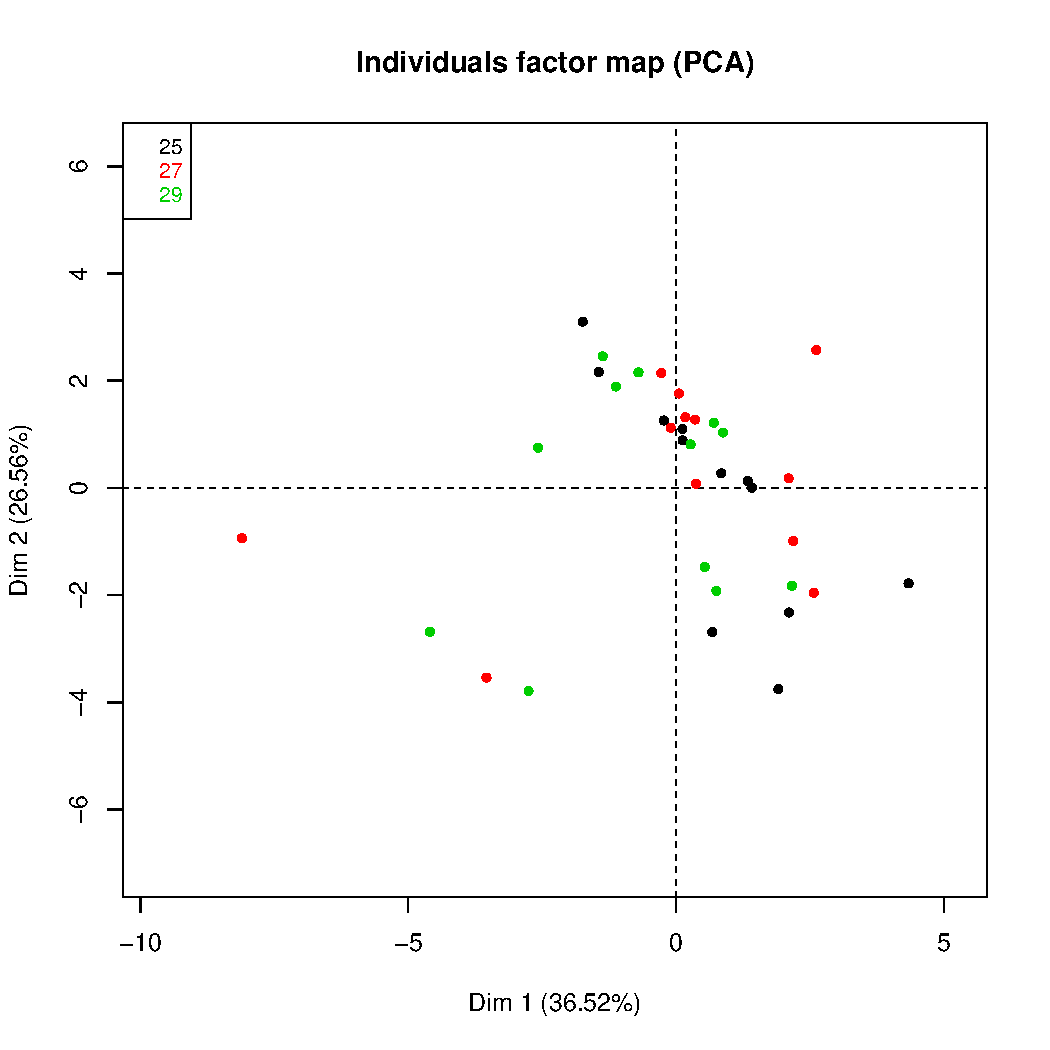
\includegraphics[width=\maxwidth]{figure/minimal-pca1-1} 

}



\end{knitrout}







\section{Discussion}


\section{Summary}
In summary, the proposed methods will help determine which features are mostly responsible for differentiating WT and mutant wells.

\section{Anticipated Results}
I expect that a subset of features will reliably distinguish the WT from the mutant wells. MEA data is, however, highly variable, therefore I expect that a prediction rate above 75 percent will be unlikely. Should there not be a classification rate above 75 percent, then I expect that the data just has too much variability to be as reliable as wished. However, understanding that our ability to distinguish WT versus mutant wells is poor will be helpful to know as well.
 happens?

\section{Conclusion}
The impact of this project will be especially helpful to understand the differences between mutant and WT wells.












\end{document}
